\documentclass{beamer}

\usepackage{graphics}
\usepackage{graphicx}
\usepackage{amsmath,amssymb,amsthm}
\usepackage{cancel}
%\usepackage{subeqnarray}
%\usepackage{easybmat}
%\usepackage{subfigure}



%\usepackage{HA-prosper}
%\usepackage[dvips,letterpaper]{geometry}

\def\Proba#1{\mathcal{P}\left(#1\right)}
\def\Surv{\mathcal{S}}
\def\R{\mathcal{R}}
\def\D{\mathcal{D}}
\def\C{\mathcal{C}}
\def\M{\mathcal{M}}
\def\L{\mathcal{L}}
\def\IC{\mathbb{C}}
\def\IN{\mathbb{N}}
\def\IR{\mathbb{R}}
\def\IZ{\mathbb{Z}}
\def\IK{\mathbb{K}}
\def\II{\mathbb{I}}
\def\Rzero{\mathcal{R}_0}
\newcommand{\diag}{\operatorname{diag}}
\def\tr{\textrm{tr}}
\def\det{\textrm{det}}
\def\sgn{\textrm{sgn}}
\def\imply{$\Rightarrow$}
\def\dbint{\int\!\!\!\int}
\def\dbintb{\mathop{\int\!\!\!\!\int}}
\def\tpint{\int\!\!\!\int\!\!\!\int}

\def\red{\color[rgb]{1,0,0}}

\def\nbOne{{\mathchoice {\rm 1\mskip-4mu l} {\rm 1\mskip-4mu l}
{\rm 1\mskip-4.5mu l} {\rm 1\mskip-5mu l}}}

\newtheorem{proposition}{Proposition}

\setbeamertemplate{navigation symbols}{}
\setbeamertemplate{footline}
{%
\quad\insertsection\hfill p. \insertpagenumber\quad\mbox{}\vskip2pt
}

\title[Identification of parameters]{Identification of parameters\\[1.5cm] Regression and Numerical integration}
\date{}

\begin{document}
\frame[plain]{\setcounter{page}{0}\titlepage}
%%%%%%%%%%%%%%
%%%%%%%%%%%%%%


\section{Statement of the problem}
\frame[plain]{\tableofcontents[current]}

\frame{\frametitle{Objective}
We are given a table with the population census at different time intervals between a date $a$ and a date $b$, and we have a model to describe the evolution of this population
\vskip1cm
We want to \textbf{find parameters} of the model so that solutions of the model \textbf{fit} the data as well as possible 
}

\frame{\frametitle{Sources of uncertainty}
\begin{itemize}
\item Some parameters are known with reasonable accuracy. Others are known within a range of possible values
\item Data is obtained through measurement, and this measurement is not necessarily very precise
\item Data is usually intrinsically ``noisy''
\item The model you have is usually wrong (\textbf{all} models are wrong, the problem is to find one that is not too wrong, i.e., capable of answering your question)
\end{itemize}
Be aware of these limitations
}

\section{Case of the logistic equation}

\frame{\frametitle{The US population from 1790 to 2000 (revised numbers)}
\begin{center}
\begin{tabular}[t]{ccc}
\begin{tabular}{cc}
Year & Population\\
& (millions) \\
\hline
1790 & 3.929 \\
1800 & 5.308 \\
1810 & 7.240 \\
1820 & 9.638 \\
1830 & 12.866 \\
1840 & 17.069 \\
1850 & 23.192 \\
1860 & 31.443 \\
1870 & 38.558 \\
1880 & 50.156 \\
1890 & 62.948
\end{tabular} 
&\quad &
\begin{tabular}{cc}
Year & Population \\
& (millions) \\
\hline
1900 & 76.212 \\
1910 & 92.228 \\
1920 & 106.021 \\
1930 & 123.202 \\
1940 & 132.164 \\
1950 & 151.325 \\
1960 & 179.323 \\
1970 & 203.302 \\
1980 & 226.542 \\
1990 & 248.709 \\
2000 & 281.421
\end{tabular}
\end{tabular}
\end{center}
}

\frame{\frametitle{The logistic equation}
$r$ the intrinsic growth rate of the population, $K$ the carrying capacity,
\begin{equation}\label{eq:ode_logistic_ident}
N'=rN\left(1-\frac NK\right)\tag{Logistic}
\end{equation}
}

\frame{\frametitle{Parameter identification}
To identify parameters, we can use \textbf{nonlinear regression}. With the logistic equation, there are two methods:
\begin{enumerate}
\item Since the solution $N(t)$ to \eqref{eq:ode_logistic_ident} is known, we can use nonlinear regression directly on $N(t)$
\item We use nonlinear regression on the constructed (simulated) solution to \eqref{eq:ode_logistic_ident}
\end{enumerate}
}

\section{Using nonlinear regression}

\frame[containsverbatim]{\frametitle{Finding the solution of \eqref{eq:ode_logistic_ident} using maple}
\begin{verbatim}
eq := diff(N(t),t) = r*N(t)*(1-N(t)/K)
\end{verbatim}
\[
\frac{d}{dt}N(t)=rN(t)\left(1-\frac{N(t)}{K}\right)
\]
Solve without specifying an initial condition:
\begin{verbatim}
dsolve(eq, N(t))
\end{verbatim}
\[
N(t)=\frac{K}{1+e^{-rt}\_C1 K}
\]
Solve with initial condition $N(0)=C$:
\begin{verbatim}
dsolve({eq, N(t0) = C}, N(t))
\end{verbatim}
\[
N(t)=\frac{CKe^{-rt_0}}{Ce^{-rt_0}+e^{-rt}K-e^{-rt}C}
\]
}


\frame{
We use the solution
\[
N(t)=\frac{N_0Ke^{-rt_0}}{N_0e^{-rt_0}+e^{-rt}(K-N_0)}
\]
(we have replaced $C$ by $N_0$)
\vskip1cm
To reduce the number of parameters to find, we assume that the initial point is $(t_0,N_0)=(1790,3.929)$, the first data point
\vskip1cm
Note that we are working in millions (this is important later)
}


\frame{
Write the points as $(t_k,N_k)$, $k=2,\ldots,22$ --there are 22 data points, but we use the first as $(t_0,N_0)$ or, to make things more convenient to write, $(t_1,N_1)$. We want to minimize
\[
S=\sum_{k=2}^{22} \left(N(t_k)-N_k\right)^2,
\]
where $t_k$ are the known dates, $N_k$ are the known populations, and \[
N(t_k)=\frac{N_0Ke^{-rt_0}}{N_0e^{-rt_0}+e^{-rt_k}(K-N_0)}
\]
}

\frame{
Emphasize dependence on $r,K$:
\[
S(r,K)=\sum_{k=2}^{22} \left(
\frac{N_0Ke^{-rt_0}}{N_0e^{-rt_0}+e^{-rt_k}(K-N_0)}-N_k
\right)^2
\]
This is maximal if (necessary condition) $\partial S/\partial r=\partial S/\partial K=0$. 
}

\frame{
We have, for a given $k=2,\ldots,22$,
\begin{multline*}
\frac 12\;\frac{\partial}{\partial r}
\left(
\frac{N_0Ke^{-rt_0}}{N_0e^{-rt_0}+e^{-rt_k}(K-N_0)}-N_k
\right)^2 = \\
\frac
{K \left( N_k (N_0-K) e^{-rt_k}+
N_0e^{-rt_0}(K-N_k)  \right) 
N_0e^{-r(t_0+t_k)}(t_0-t_k)(N_0-K) }
{ \left( N_0{e^{-rt_0}}+{e^{-rt_k}}(K-N_0)  \right) ^3}
\end{multline*}
and
\begin{multline*}
\frac 12\;\frac{\partial}{\partial K}
\left(
\frac{N_0Ke^{-rt_0}}{N_0e^{-rt_0}+e^{-rt_k}(K-N_0)}-N_k
\right)^2 = \\
\frac 
{\left(e^{-rt_0}-e^{-rt_k}\right)  
\left(N_k(N_0-K)e^{-rt_k}+N_0e^{-rt_0}
(K-N_k)  \right) {N_0}^2{e^{-rt_0}}}
{\left(N_0e^{-rt_0}+e^{-rt_k}(K-N_0)\right)^3}
\end{multline*}
}

\frame{
So $\partial S/\partial r=0\Leftrightarrow$
\[
\left(N_k (N_0-K) e^{-rt_k}+N_0e^{-rt_0}(K-N_k)\right) 
N_0e^{-r(t_0+t_k)}(t_0-t_k)(N_0-K)=0
\]
(provided $\left(N_0{e^{-rt_0}}+{e^{-rt_k}}(K-N_0)\right) ^3\neq 0$)
\vskip0.5cm 
That is $\partial S/\partial r=0\Leftrightarrow$
\begin{equation}\label{eq:constraint1_regression}
N_k (N_0-K) e^{-rt_k}+N_0e^{-rt_0}(K-N_k)=0 \tag{*}
\end{equation}
or
\[
t_0-t_k=0\qquad\textrm{or}\qquad N_0-K=0
\]
The case $t_0=t_k$ cannot happen, since $k=2,\ldots,22$ (and we assume we do not have two different measurements for one time value). So we have either $K=N_0$ or \eqref{eq:constraint1_regression}
}

\frame{
Solving \eqref{eq:constraint1_regression} for $r$, we get
\[
r=-\frac{\ln\left(\frac{N_0(K-N_k)}{N_k(K-N_0)}\right)}{t_k-t_0}
=\frac{\ln\left(\frac{N_k(K-N_0)}{N_0(K-N_k)}\right)}{t_k-t_0}
\]
}

\frame{
Also $\partial S/\partial K=0\Leftrightarrow$
\[
\left(e^{-rt_0}-e^{-rt_k}\right)  
\left(N_k(N_0-K)e^{-rt_k}+N_0e^{-rt_0}
(K-N_k)  \right)=0
\]
(provided $\left(N_0e^{-rt_0}+e^{-rt_k}(K-N_0)\right)^3\neq 0$)
\vskip0.5cm
That is, $\partial S/\partial K=0\Leftrightarrow$
\[
e^{-rt_0}-e^{-rt_k}=0
\]
or
\begin{equation}\label{eq:constraint2_regression}
N_k(N_0-K)e^{-rt_k}+N_0e^{-rt_0}(K-N_k)=0\tag{**}
\end{equation}
The first condition implies $t_0=t_k$, which is impossible. So we are left with \eqref{eq:constraint2_regression}, which is the same equation as \eqref{eq:constraint1_regression}
}

\frame{
So this is a difficult problem.. (see the theory for nonlinear least squares if you are interested)
\vskip1cm
So we use plan B: numerics directly..
}


\section{Using simulations}

\frame{\frametitle{What we need to do}
Let us forget that we know the explicit solution to \eqref{eq:ode_logistic_ident}
\vskip0.5cm
\begin{itemize}
\item The solution to \eqref{eq:ode_logistic_ident} can be approximated numerically
\item We can construct one such numerical solution for given values of $r$ and $K$
\item We then can see ``how far off'' that solution is from our data points
\item We change the parameters $r$ and $K$ a little, find out ``how far off'' the new solution is from the data points
\item And repeat until we have found a solution that is better than others..
\end{itemize}
}


\frame{\frametitle{Finding the numerical solution to \eqref{eq:ode_logistic_ident}}
We can use
\begin{itemize}
\item matlab
\item octave
\item scilab
\item maple
\item mathematica
\item many others..
\end{itemize}
matlab, octave and scilab are recommended because of the ``philosophy''
}


\frame{\frametitle{Using matlab}
In matlab (and octave) the philosophy is very close to the ``natural'' way one proceeds with an ode: given the ODE
\[
x'=f(t,x)
\]
we must define the right hand side (RHS) function (the vector field) $f(t,x)$, and use it to compute the (numerical) solution
}

\frame{\frametitle{Reminder: Euler's method}
The solution to the initial value problem
\begin{align*}
x' &= f(t,x) \\
x(t_0) &= x_0
\end{align*}
can be approximated numerically by the following sequence:
\begin{align*}
t_{k+1} &= t_k+h \\
x_{k+1} &= x_k+hf(t_k,x_k)
\end{align*}
for a time step $h>0$ and with first term $(t_0,x_0)$
}


\frame{\frametitle{Back to matlab}
The techniques (a.k.a. ``numerical solvers'') in matlab are much more advanced, but the idea is the same: approximate the solution to an ODE by using a numerical algorithm the uses information on the ``shape'' of the vector field
\vskip0.5cm
We need two files:
\begin{enumerate}
\item a RHS function defining $f(t,x)$
\item a function or command line statement that ``calls'' the RHS function with a numerical solver
\end{enumerate}
}


\frame[containsverbatim]{\frametitle{The RHS function}
For the logistic equation, we could define the following function
\begin{verbatim}
function dN=rhs_logistic(t,N,p)
% This function returns the value of dN/dt 
% at the point (t,N), using parameters in the 
% structure p

dN=p.r*N*(1-N/p.K);
\end{verbatim}
which we save in a file called, say, \verb%rhs_logistic.m%
\vskip0.5cm
Note that {\tt t} is required in the function arguments even if not used in the RHS function, i.e., even if $f$ is autonomous
}

\frame[containsverbatim]{\frametitle{Using structures}
The variable {\tt p} is defined as a \emph{structure}. This is a very useful construct in many programming languages. Think of it as a \emph{container}:
\begin{verbatim}
>> p.K=100;
>> p.r=2;
>> p
p =
    K: 100
    r: 2
\end{verbatim}
Pros: {\tt p} is passed to the function as one parameter, instead of a list of parameters. Cons: do not forget {\tt p.} in front of the parameter
\vskip0.5cm
We will see later why structures are useful
}

\frame[containsverbatim]{\frametitle{Invoking the numerical solver}
The call is of the form (from the help): 
\begin{verbatim}
ode23, ode45, ode113, ode15s, ode23s, ode23t, ode23tb

Solve initial value problems for ordinary differential 
equations

Syntax
[T,Y] = solver(odefun,tspan,y0)
[T,Y] = solver(odefun,tspan,y0,options)
[T,Y,TE,YE,IE] = solver(odefun,tspan,y0,options)
sol = solver(odefun,[t0 tf],y0...)

where solver is one of ode45, ode23, ode113, ode15s, 
ode23s, ode23t, or ode23tb
\end{verbatim}
Typically, you can use {\tt ode45}
}


\frame[containsverbatim]{\frametitle{Computing the numerical solution to the logistic}
We call our solver as follows:
\begin{verbatim}
tspan=[1790 2000]; %The time span of the solution
IC=3.929;          %The initial condition (in 1790)
p.K=300;           %Set the parameters
p.r=0.5;
[t,N]=ode45(@rhs_logistic,tspan,IC,[],p);
\end{verbatim}
(The one before last argument, {\tt []}, represents the options structure. Here we are not modifying any option, and so pass an empty vector)
\vskip0.5cm
Save this file as, say, \verb%call_solver.m% 
\vskip0.5cm
After running it, we have a vector {\tt t} of times (covering {\tt tspan}) and a vector {\tt N} of solution
}

\frame[containsverbatim]{\frametitle{Plotting the solution}
\begin{verbatim}
plot(t,N)
\end{verbatim}
gives
\begin{figure}[htbp]
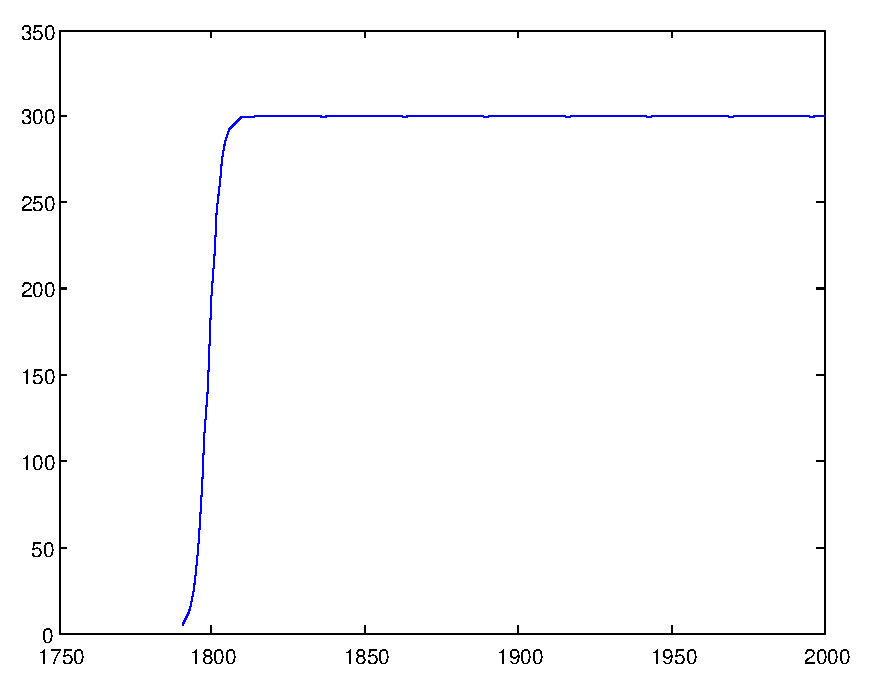
\includegraphics[width=0.7\textwidth]{../figs_09_parameter_identification/fig_logistic_ode_1}
\end{figure}
}

\frame[containsverbatim]{\frametitle{Tightening the $x$-axis}
\begin{verbatim}
plot(t,N)
xlim([t(1) t(end)])
\end{verbatim}
gives
\begin{figure}[htbp]
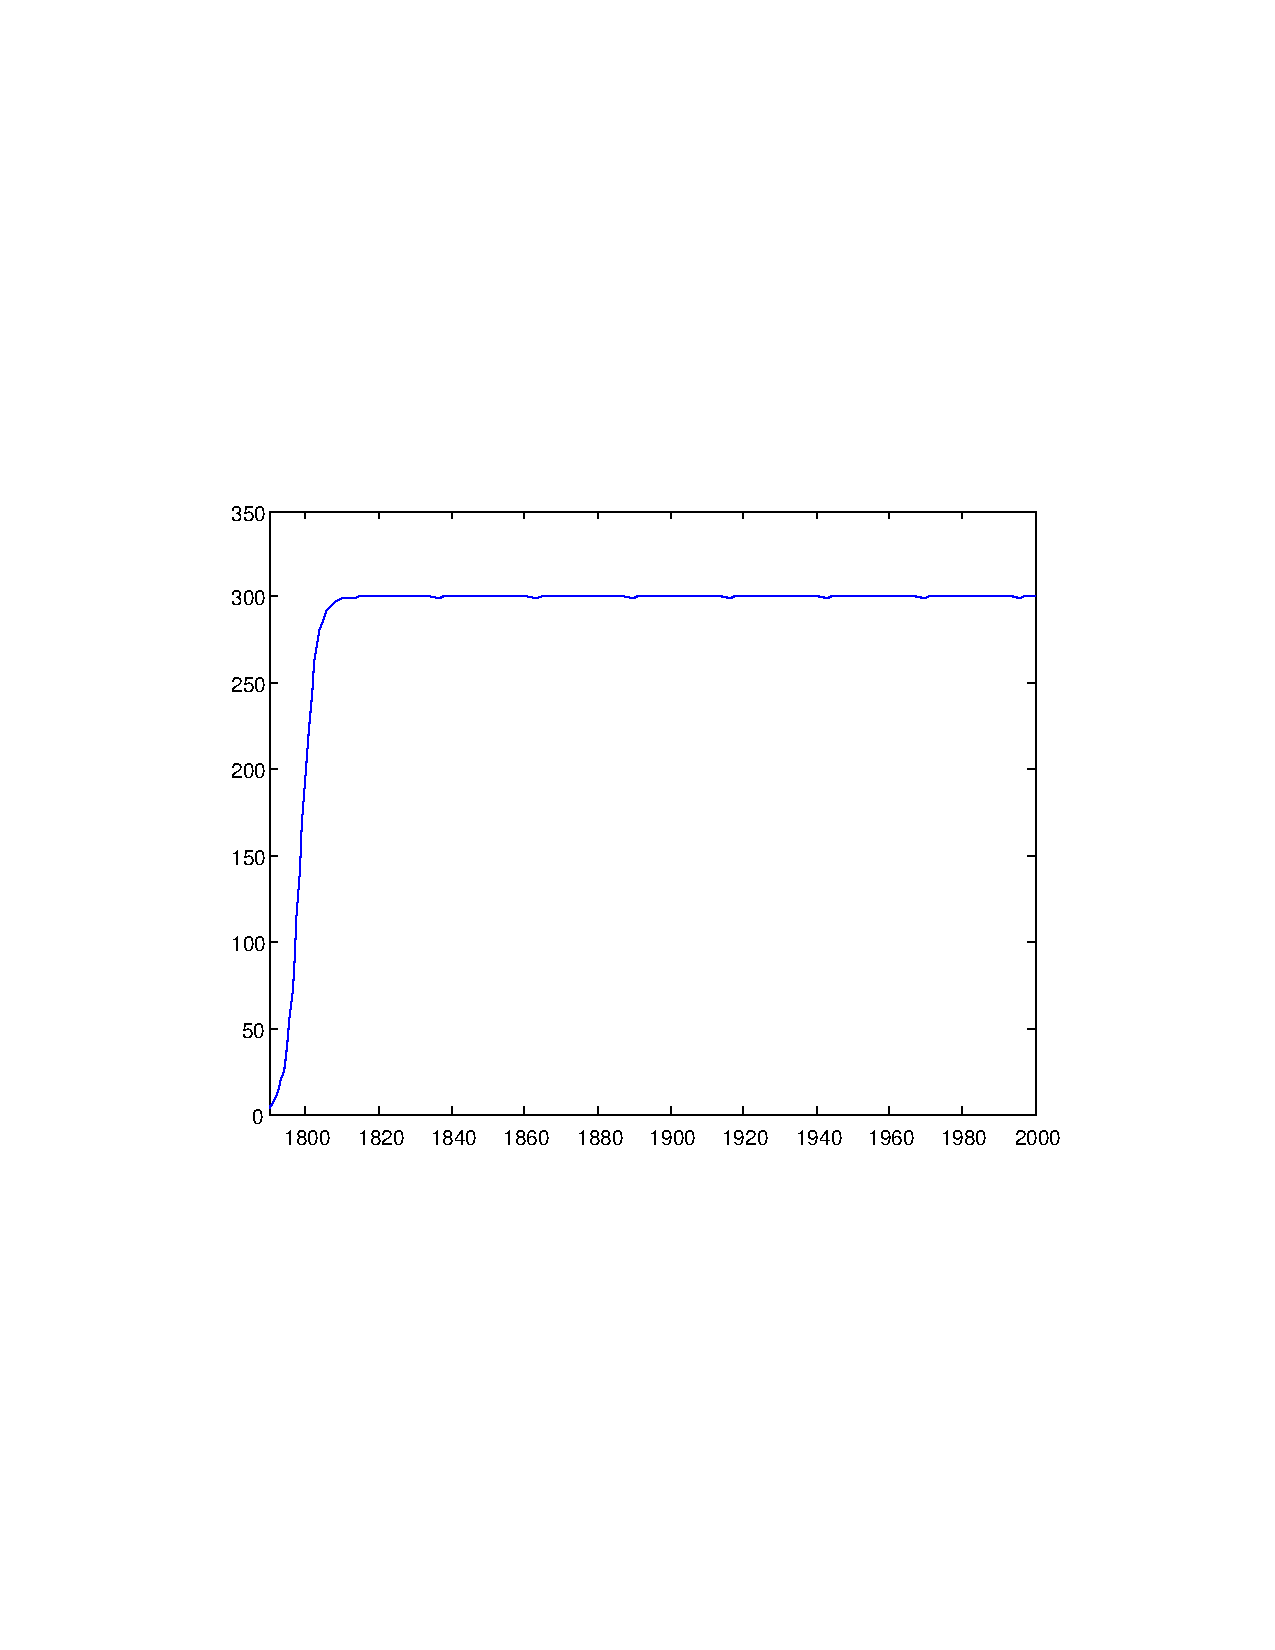
\includegraphics[width=0.7\textwidth]{../figs_09_parameter_identification/fig_logistic_ode_2}
\end{figure}
}

\frame[containsverbatim]{\frametitle{Using Octave}
The syntax in Octave is almost identical to the matlab syntax. In fact, if you use the additional programs in the {\tt forge} repository, a function {\tt ode45} is defined
\vskip0.5cm
However, the functions (in octave) do not implement the use of a parameter by default, so a work-around must be used
\vskip0.5cm
Update: as of V3.0 and using ode45, parameters can be passed and the matlab code given before works, with the following little modification:
\begin{verbatim}
opt=odeset('InitialStep',0.05,'MaxStep',1);
[t,N]=ode45(@rhs_logistic,tspan,IC,opt,p);
\end{verbatim}
which makes sure that the time step does not become too large)
}


\frame[containsverbatim]{\frametitle{Using scilab}
The syntax in scilab differs a little from matlab, so beware.
\begin{verbatim}
function ydot=f(t,y);
ydot=y^2-y*sin(t)+cos(t);
endfunction
\end{verbatim}
}





\end{document}